\section{Увод}

\subsection{Триизмерно пространство}
Триизмерното пространство (3D) е геометричен 3-параметров (x, y, z) модел на физичния свят. Той се отбелязва със симовла ${\rm I\!R^3}$. Използваме този модел в компютърната графика за математическото обяснение на 3D предметите в пространстовото, съответно визуализацията им.

\begin{center}
\begin{figure}[h]
    \centering
    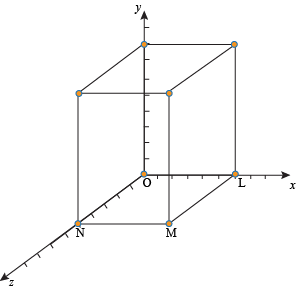
\includegraphics[width=120pt]{3dcube.png}
    \caption{Паралелепипед в тримерно пространство}
    \label{fig:mesh1}
\end{figure}
\end{center}

\subsection{3D Модел}
3D моделите са математическа репрезентация на триизмерен обект. Могат да бъдат изразени чрез данни в триизмерна координатна система. Един от начините е да се описват по сравнително груб начин чрез воксели. Вокселите са стойности в грид в триизмерното пространство, опитвайки се да бъдат еквивалента на 3D пиксели. 

\begin{figure}
\centering
\parbox{5cm}{
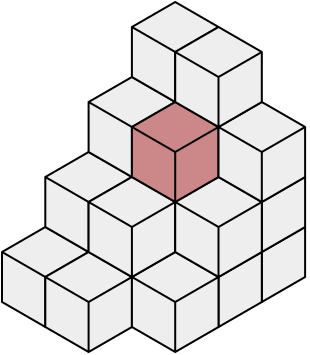
\includegraphics[width=4cm]{voxels.png}
\caption{Воксели}
\label{fig:2figsA}}
\qquad
\begin{minipage}{5cm}
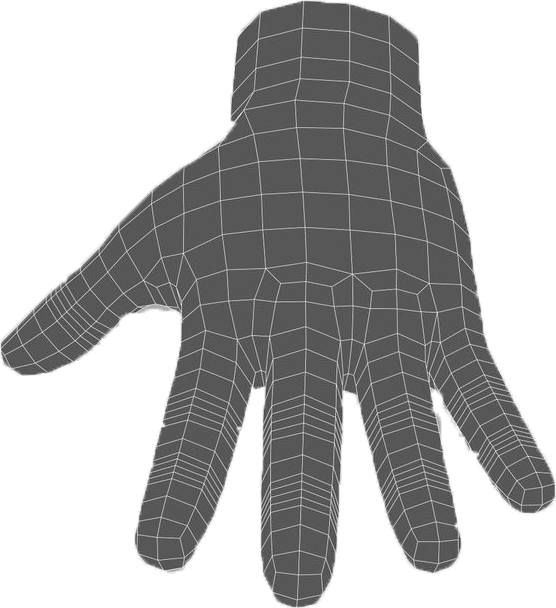
\includegraphics[width=4cm]{hand.png}
\caption{Модел на ръка}
\label{fig:2figsB}
\end{minipage}
\end{figure}

Вокселите в по-високи резолюции изискват много повече компютърна калкулация за изкуствено генериране. Което лимитира учените до модели с ниска резолюция.
В повечето случаи обаче, 3D моделите могат да бъдат означени с върхове, лица и съответно полигони(площта на 3 или повече свързани върха) образувани от тях. Триизмерните фигури са фундаментална част от индустрията на 3D игрите, анимациите, физическите симулации и архитектурата.

\subsection{Същност/Идея}

CiD (рекурсивен акроним за CiD is Deep) разглежда разлчини подходи към проблема за генериране на 3D модели/повърхности изразени чрез върхове, лица и полигони вместо досега изследваните чрез Воксели. 
3D Моделите ще са базирани на $K$ на брой модела с подобни характеристики на зададените от потребителя параметри.

\section{Проблемът}
Задачата на която се търси решение е генерирането на 3D модели/повърхности по зададени от потребителя параметри, на базата на други. Като главната идея зад намирането на оптимален модел, сходен на истинсиките, но запазвайки смисъла и определението си (когато се иска маса да се получава маса). Затова Машинното самообучение бе избрано като подход. Потребителят заявява, че иска ``маса'' с допълнителни тагове ``school'' и ``office'' и ще се селектират $K$ на брой възможно най-отговарящи на заданието модели на маса, чрез алгоритъмa $K-Nearest Neighbors$. Тези $K$ на брой модели ще бъдат входни данни на трениран модел от невронни мрежи, който ще генерира подходяща повърхност/обект според зададените тагове. Техническите детайли те първа ще подлежат на описание по-надолу в документацията.
\section{Приложимост}

Изследването по темата е силно приложимо в CGI (Computer Generated Imagery)/CAD (Computer Aided Design)/ Gaming индустрията.

\subsection{Royalty Free}
Създателите на игри, филми, дизайн на жилища или анимации ще могат да генерират определени 3D модели според изискванията си за дадената задача. Това ще ускори сериозно прототипизирането на продукти, което цялостно би скъсило времето за реализиране на даден проект, съответно и цената му. Също така генерираните модели ще бъдат Royalty Free, което ги прави напълно използваеми за академични и комерсиални цели.

\subsection{Потенциален бизнес план}
В последствие на времето при положителни резултати, това ще се направи под формата на достъпна за всички, уеб платформа в която хората ще могат да генерират, споделят и обсъждат своите Royalty free 3D модели. След определен брой free 3D генериране на модели, ще се иска месечна такса или на брой.

\section{Какво е Невронна Мрежа? Нотация}
\subsection{Същност}

Невронна мрежа, е модел за обработка на информация, вдъхновен от изучаването на биоелектричните мрежи в мозъка на човека и животните. Тя се състоят от свързани неврони и обмяна на синапси (импулси) помежду им. Могат да се учат, взимайки предвид различни примери и да решава задачи като: да анализира голям брой снимки с етикети ``Куче'' и ``Не куче'', след като си направи ``изводите'', научената мрежа може да се използва за разпознаване на кучета в други снимки. Най-използвани са за проблеми които се изразяват трудно чрез специфично уравнение или алгоритъм.
\begin{center}
\begin{figure}[h]
    \centering
    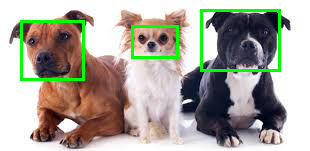
\includegraphics[width=250pt]{dogs.png}
\end{figure}
\end{center}
Всеки неврон приема сигнали (означени с $x_i$, където $i$ значи $i$-тия неврон) от другите свързани към него (под формата на числа). Всяка връзка има тегло (означено с $w_j_i$, като $j,i$ означава $j$-тата тежест на $i$-тия неврон), която, умножавайки се със сигнала, определя неговата значимост. Понеже само с умножение, една мрежа в повечето случай ще бъде просто калкулатор за матрици и няма да върши реална сложна работа без Биас (отбелязваме го с $b$). Той служи за наместване на кога ще се активира даден неврон според задачата която му е дадена. След това импулсът на прост персептрон (един неврон), изглежда по следния начин, като $n$ стои за броя на неговите входни неврони:

\begin{center}
\[ \sum_{i=1}^{n} (w_i*x_i) + b = output\]
\end{center} 

След което изхода минава през активационна функция. Тя "сплесква" изхода в число между 0 и 1. Използва се главно ReLU (Rectified Linear Unit) за активация:

\begin{center}
$f(x)=\max(0,Х)$
\end{center}

чиито изход се препраща към другите неврони или към себе си в зависимост от връзката, типa на мрежата и/или други параметри. Най-често, невроните са организирани в слоеве:

\begin{center}
\begin{figure}[h]
    \centering
    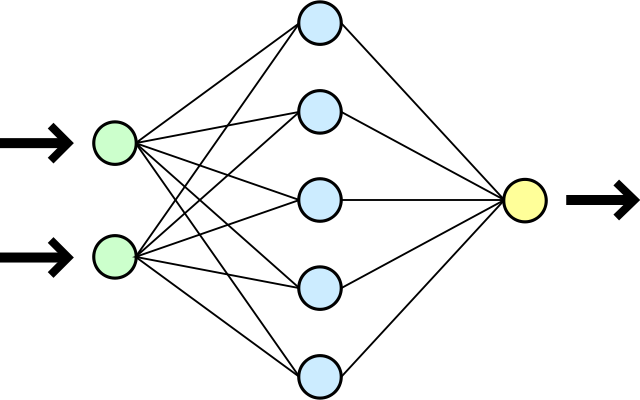
\includegraphics[width=180pt]{network1.png}
    \caption{Невронна мрежа с 1 входен слой от 2 неврона, 1 скрит слой от 5 неврона и 1 изходен неврон.}
    \label{fig:mesh1}
\end{figure}
\end{center}

Един от по-известните видове невронни мрежи, се наричат конволюционни. Те се ползват за класифициране и разпознаване на снимки. Състоят се от три вида невронни слоя: Входен (Input), Скрит (Hidden), Изходен (Output) както е показано на Фигура 4. Входният слой се използва за вкарване на пъвоначалните данни, Скритите слоеве се ползват за да оформят входните данни във формат, който изходния слой може да използва за да даде крайно решение за текущото състояние на мрежата - да класифицира дадена снимка примерно. Тренирането на една мрежа се случва, като изходния слой изчислява грешката, като $f({\vec {x}})$ изхода и $y$ e очаквания резултат от данните с които се тренира текущата итерация. Пример за обикновена Loss функция:

\begin{center}
$Loss(f({\vec {x}}),y)=(f({\vec {x}}) - y)^{2}$
\end{center}

Грешката се връща назад в мрежата чрез главните алгоритми които позволяват стоят в ядрото на невронните мрежи: Backpropagation (предава грешката обратно по невроните за да знаят как да се коригират, според това от кой зависи най-много) и оптимизатори като Gradient Descent (стъпките до възможно най-ниската грешка).

\subsection{Защо Невронните Мрежи са толкова популярни?}
Невронните мрежи са открити още през 1944 от Warren McCullough.
В днешно време те могат да се използват за огромно множество от проблеми. На теория всичко което може да се представи с числа е подходящ сет от данни за решението на даден проблем. Защо чак сега? Главната причина е бързото развитие на компутационните устройства (computation units) по-точно видеокартите(GPUs). Навлизат с все по-добро съотношение цена:сила. Главното им качество е, че могат да смятат/умножават десетки пъти по-бързо от процесорите(CPUs) матрици,вектори, което е в основата на невронните мрежи и правят достъпно по-интензивно и по-продължително трениране.

\subsection{Недостатъци}
Компютърната мощ, въпреки по-достъпна, все още е изключително го-лям фактор, особено в задачи като тази, в които се работи със снимки, тримерни повърхности или като цяло огромно количество данни. Главната дилема в решението на повечето проблеми със машинно самообучение е недостигна данни. Данните имат директен ефект върху резултатите без значение колко бърз или ефективен е даден алгоритъм. Разбира се резултатите могат да се подобрят с по-оптимални за дадения проблем алгоритми или подобрение на самия формат и моделиране на данните, при условие че има данни, които отговарят до някаква степен на критериите посочени според задачата.

\section{Данни}

Данните както стана ясно са един от главните проблеми за решаване при подход с машинно самообучение/невронни мрежи. За реализацията на този проект, трябва именуван, добре структуриран и разбираем от невронната мрежа сет от данни включващи всякакви 3D модели. 

\subsection{Източници}
На пръв поглед изглеждайки невъзможно след известно търсене се стигна до датасет-а ScanNet, който съдържа 1500 сканирани стаи с $2,500,500$ гледни точки общо. Това за жалост не върши работа, при условие че се иска генерирацията на единични 3D обекти. След още търсене, се попадна на $ShapeNet[1]$. 30GB датасет който съдържа 52,000 модела на различни, класифицирани обекти по имена и тагове. На пръв поглед изглежда перфектно, но не е достъпен за всички. Изискваше да се подаде заявка, която администраторите преглеждат преди да дадат права на даден човек да изтегли датасет-а. Заявката съдържа какво се смята да се прави с датасет-а и в моя случай отне 3 седмици докато бъде приета, което забави значително прогреса на изследването.\\

%\begin{center}
%\begin{figure}[h]
%    \centering
%    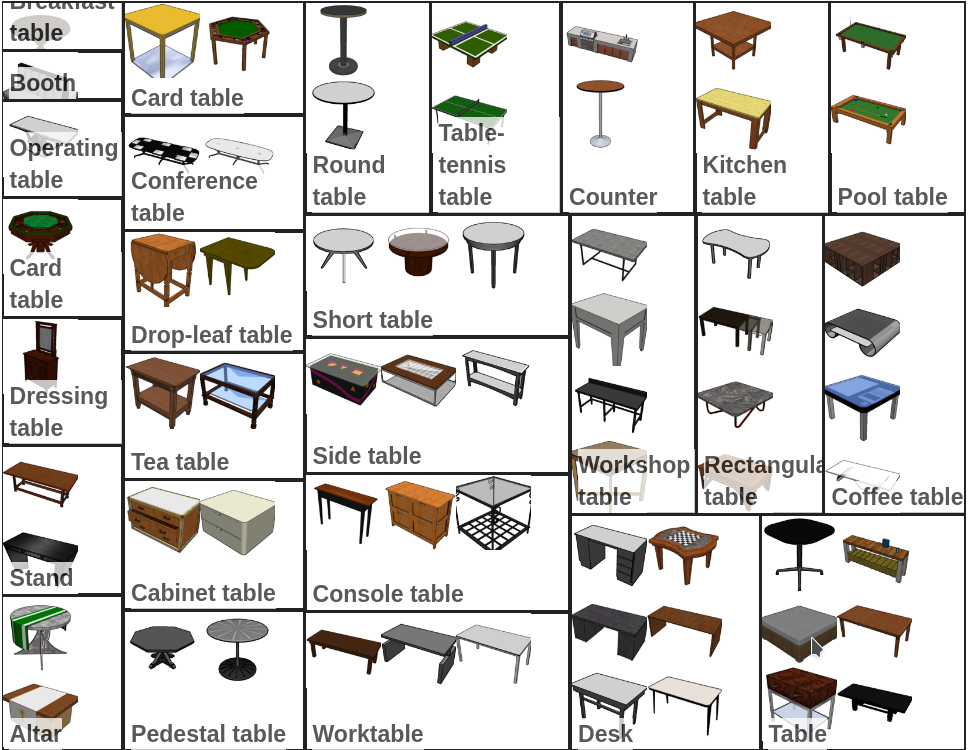
\includegraphics[width=310pt]{shapenetdata.png}
%\end{figure}
%\end{center}
\newpage
\subsection{Формати}
Какво се има предвид под ``разбираем от невронната мрежа'' формат?\\
Всички данни са във формат $.obj$, където всички върхове (vertices), лица (faces) и текстури (textures) са описани по следния начин ($\#$ значи коментар):

\begin{lstlisting}
    #Vertices
    v 0.123 0.234 0.345 1.0
    #Textures
    vt 0.500 1 [0]
    # List of vertex normals.
    vn 0.707 0.000 0.707
    # Parameter space vertices
    vp 0.310000 3.210000 2.10000
    # Polygonal face element
    f 1 2 3
    f 6/4/1 3/5/3 7/6/5
    f 7//1 8//2 9//3
\end{lstlisting}
\textbf{Формати:}\\
Върхове (v): $(x,y,z[,w])$ координати, $w$ не е задължителен параметър, по подразбиране е 1.0\\
Текстури (vt): $(u, v [,w])$ координати, те са между 0 и 1, $w$ не е задължителен и по подразбиране е 0 \\
Нормали на върховете (vn): $(x,y,z)$ координати; Нормалите не е задължително да са базови вектори (unit vectors). \\
Пространствени параметри, използват се за означаване на точки в извито пространство (vp): $(u[,v][,w])$ формат.\\
Лица/Полигони (f): $\hspace{1mm}v_1\hspace{1mm}v_2 \hspace{1mm}v_3$ формат, като $v_i$ е връх.
Описаният по-долу подход подлежи на допълнитлно изследване и доказаване.

\subsubsection{Подход}

Понеже всичко е репрезентирано като точка в пространството. Възможно е да се напише парсер който да извлече данните. И всичко да се конвертира във нормали на върхове и лица - вектори, които след конкатенация стават матрици, които невронните мрежи ще разбират.\\

Главният проблем в такъв случай ще е декодирането на изхода от невронната мрежа. Предполага се че мрежата ще запази структурата на входа. Това би значело, че ако първите няколко колонки на една входна матрица значат нормал на връх ($v^j_i$, което в случая ще означа като координати по оста $j$ и индекс на вектора $i$), a останалите, на лица ($f^j_i$), в изхода трябва да е във формāта на дадения вход също. Пример за формат:

\[ \left( \begin{array}{ccccccc}
v^x_1 & v^x_2 & v^x_3 & f^x_4 & f^x_5 & f^x_6 & f^x_7\\
v^y_1 & v^y_2 & v^y_3 & f^y_4 & f^y_5 & f^y_6 & f^y_7\\
v^z_1 & v^z_2 & v^z_3 & f^z_4 & f^z_5 & f^z_6 & f^z_7\\
v^w_1 & v^w_2 & v^w_3 & 0 & 0 & 0 & 0
\end{array} \right)
\]
\begin{center}
\begin{figure}[h]
    \centering
    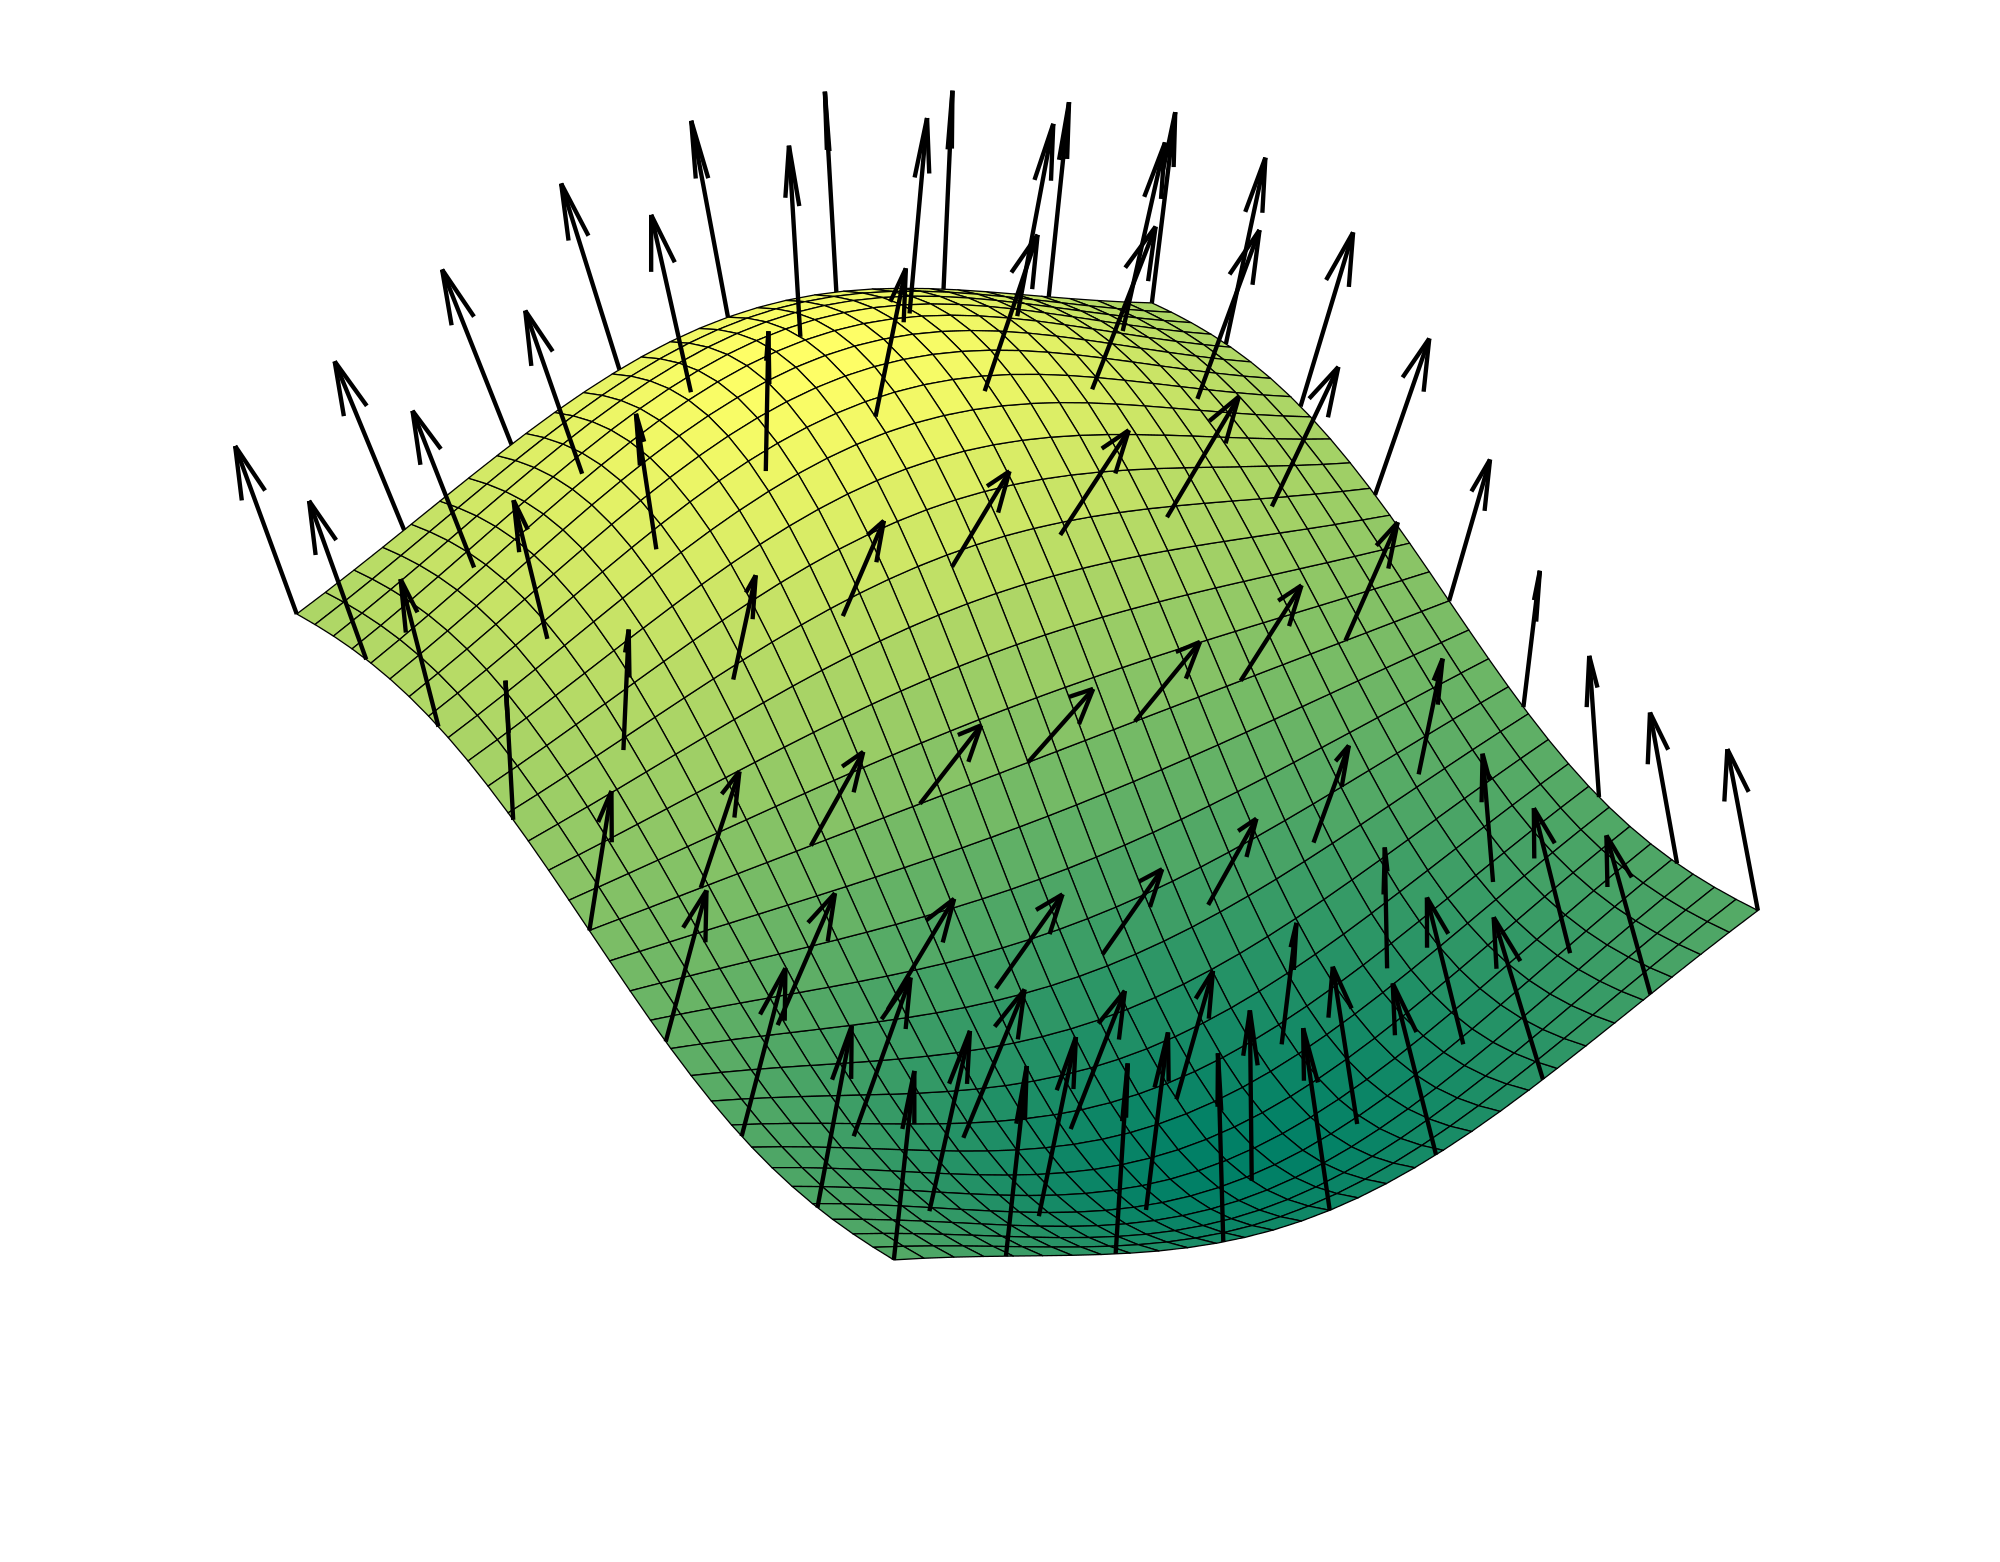
\includegraphics[width=300pt]{normals.png}
    \caption{Нормали на извита повърхност}
    \label{fig:mesh1}
\end{figure}
\end{center}
Калкулиране на нормали за прости повърхности. Прост пример за триъгълник $p_1, p_2, p_3$:

\begin{center}
$\vec{U} = p_2 - p_1 \hspace{0.5in} \vec{V} = p_3 - p_1\\
N_x = \vec{U}_y*\vec{V}_z - \vec{U}_z*\vec{V}_y\\
N_y = \vec{U}_z*\vec{V}_x - \vec{U}_x*\vec{V}_z\\
N_z = \vec{U}_x*\vec{V}_y - \vec{U}_y*\vec{V}_x\\
\vec{N} = \left( \begin{array}{c}
N_x\\
N_y\\
N_z
\end{array} \right)
$
\end{center}
Формула за намиране на нормали на тримерни имплицитно определни повърхности:
\[\Large \hat{n} = \frac{\nabla F}{\sqrt{F^2_x + F^2_y + F^2_z}}\]
Където $F(x,y,z)$ е дефинирана тримерна повърхност.

\subsection{Моделиране на данни}

Моделирането на данни е от изключителна важност за резултатие на един модел от невронни мрежи. Данните ще бъдат разделени в три части за да се предотврати overfitting - този метод се нарича кръстосана валидация (cross-validation). Overfitting на един модел, интуитивно казано, е когато той се справя изключително добре на данните които е трениран, но не е успял да се генерализира за решаването на проблема. Трите части ще са разделени по следния начин валидация:тест:трениране -> 1:2:7 (Общо модели ~52,000)

\begin{center}
\begin{figure}[h]
    \centering
    \includegraphics[width=250pt]{datasplit.png}
    \caption{Съотношение м/у валидация, тест и данни за трениране}
\end{figure}
\end{center}

Допълнителна обработка също изискват данните за k-NN алгоритъм-а, който е обяснен по-надолу. Прекалено много измерения на данните могат да доведат до неточни, неконсистентни резултати.
Обрабтоката ще се състои главно в данните за таксономия/метадата (етикети, данни за класификация)  Архитектурата на един запис:

\begin{lstlisting}
   fullId,category, wnsynset, wnlemmas, up-normal-vector, front-normal-vector, units, aligned.dimensions, isContainerLike, surfaceVolume, supportSurfaceArea, weight, staticFrictionForce, name, tags
\end{lstlisting}

Както се вижда, има много данни, които не ми помагат по никакъв начин за алгоритъма kNN и биха имали негативен ефект над резултатите, затова всички колони освен $category, name, tags$, няма да се взимат в предвид.
\section{Архитектура}
\begin{center}
\begin{figure}[h]
    \centering
    \includegraphics[width=400pt]{arch.png}
\end{figure}
\end{center}
\section{Weighted k-Nearest Neighbors Алгоритъм}
k-Nearest Neighbors (kNN) е метод за класификация и регресия.

\subsection{Базов Алгоритъм}
Да кажем, че потребителят избере, че иска маса с тагове ``Tea table'' и ``Desk'', нека го означим със $C$. Има n на брой стола с подобни характеристики. За да намерим най-сходните до избора на потребителя, просто измерваме разстоянието от неговият вход, до най-близките $k$ точки, в случая нека бъдат 4. След като се установи кои са съседите, се гласува според класа им, като всеки има тежест според разстоянието от поисканата класификация.\\
\begin{center}
\begin{figure}[h]
    \centering
    \includegraphics[width=150pt]{knn.png}
\end{figure}
\end{center}
В случая ще бъде червено, защото гласовете са 2 на 2, но червените са малко по-близо.
Разстоянието може да бъде Евклидово или Манхатаново (подред) като $p$ и $q$ са точки в съответните пространства:
\begin{center}
$d(\mathbf {p},\mathbf {q})=\sqrt{\sum_{i=1}^n (q_i-p_i)^2}$\\
$d(\mathbf {p} ,\mathbf {q} )=\sum _{i=1}^{n}|p_{i}-q_{i}|$\\
\end{center}

\subsection{Добавяне на тегла}
Добавянето на тегла подпомага правилната класификация и консистентност на алгоритъма. Това става просто като добавим тежест на всеки $k$ най-близки съседа = $1/i$, където $i$ значи $i$-тия най-близък съсед. Това води до: $\sum _{{i=1}}^{n}w_{{ni}}=1$

\newline
\section{Експерименти}
\subsection{Генеративна Състезателна Мрежа}

\begin{wrapfigure}{r}{5.9cm}
\includegraphics[width=5.9cm]{gan2.png}
\end{wrapfigure} 

%------------------------------------------
Чрез тези модели, са постиганти някои много добри резултати в сферата на компютърната визия и генерирането на видео, затова ми е интересно как този интересен модел би се справил с задачата да генерира 3D повърхности. При това при този модел мрежи не се изискват етикети (labels), което представлява възможността да се генерализира в генерацията, понеже моделите могат да се вкарват без допълнителна човешка намеса, стига да са в същия входен формат.

%------------------------------------------

%------------------------------------------
\subsubsection{Архитектура}
Мрежата се състои от мрежа генератор $G(x)$ и от мрежа дискриминатор $D(x)$.
Генераторът, взима латентен вектор със случайни стойности $z$ и генерира единица данни, които се предават напред към дискриминатора. Той взима генерираният сампъл и истинските данни, след което ги сравнява и решава дали генераторът е изкарал достоверна единица данни. Дискриминаторът в повечето случай прави точно обратното на генератора, взима единица данни и го свежда до вектори.

\subsubsection{Трениране}
Тренирането на този вид мрежи е най-големият им недостатък. Те се състезават, като всяка отделно става все по-добра в това което прави. Дискриминаторът да решава дали генерирани единици данни са достатъчно автентични, че да ги нарече ``истински'', а Генераторът да успява да заблуди дискриминатора с все по-детайлни и автентични данни. Това би било единственият проблем по-отношение на използването на този модел и подлежи на 

\subsubsection{Loss Функция}
Изходите от генератора и дискриминатора влизат в свои loss функции:
\begin{center}
$
DLoss = \nabla \theta_d \frac{1}{m} \sum_{i=1}^m (logD(x^{(i)}) + log(1-D(G(z^{(i)})))\\
GLoss = \nabla \theta_g \frac{1}{m} \sum_{i=1}^m log(1-D(G(z^{(i)}))
$
\end{center}

$\nabla \theta_d$ и $\nabla \theta_g$ са съответно градиентите на дискриминатора и на генератора, $m$ е големината на пакетите (batch) от данни с които тренираме. Идеята зад $DLoss$ е вероятността на истинските данни $D(x^{(i)})$ да има винаги по-голяма тежест над крайното решение. Ролята на $log$ в тези Loss функции е мащабируемост и да улесни работата на компютъра драстично, като не го кара да смята числа с 20 символа след десетичната запетая. $D(G(z^{(i)}))$ значи че изхода от генератора, вкарваме в дискриминатора. Това го изкарваме от числото 1 за да получим вероятност.

\subsection{Остатъчна невронна мрежа}
Изключително нов модел, който се справя със всякакви задачи до момента. Различава се от другите със свойството да бъде много по-дълбок, без да губи ефективност в ученето. Способността на този модел е много висока и засега се справя във всякакви сфери, разпознаване на снимки, до разпознаване на гласове. Затова смятам, че бъдещите опити с нея са обещаващи.

\subsubsection{Архитектура}
Така изглежда един строителен блок (building block) на остатъчна невронна мрежа.
\begin{center}
\begin{figure}[h]
    \centering
    \includegraphics[width=250pt]{residuallayer.png}
\end{figure}
\end{center}

\subsubsection{Трениране}

Тази малка модификация, да се добави идентичност, осигурява че следващият слой със сигурност ще научи нещо повече от този, защото той получава не само, наученото от този, но и първоначалния му вход. Това позволява наслагването на много блокове един върху друг без губене на ефективност в ученето. Подобни връзки между невроните (приличат си с тези на LSTM клетките, но без порти (gates)) са решение на проблема за изчезващия градиент (vanishing gradient), който в противен случай е голяма пречка на един модел в дадени ситуации.

\section{Състояние на разработката}
Проектът е главно на идейно и теоретично ниво все още поради множество фактори, но е в бърз и обещаващ процес на разработка и може да се следи на $https://github.com/VikVelev/CiD$

\section{Техническа Реализация}
\subsection{Технологии}

За разработката на проекта ще се ползва Tensorflow като библиотека за Machine Learning. Беше избрана според наличието на интернет ресурси, документация и популярност (Community support). Интегриран Git за контрол над версиите. Pyenv за контролиране на dependency-та и по-чист поток на работа. Docker за пълна съвместимост с всякакви машини.
За писане, тестване и дебъгване на математиката зад генерирането ще се ползва PyOpenGL.

\begin{center}
\begin{figure}[h]
    \centering
    
\includegraphics[width=330pt]{dockertf.png}
\end{figure}
\end{center}

\subsection{Математика}
Преди навлизането в Машинното Самообучение, не бях запознат с по-голямата част от математиката, която стои зад тях (Диференциали, Интеграли, ЛААГ). Това отнема сериозно количество време, което е неизбежно за реализацията на този проект.
\subsection{Компютърна мощ}
Поради огромния датасет и жанра на проблема, се изисква мощ в големи количества, за ефективен поток на работа, и достигане на адекватни резултати по-ефективно и бързо.
\section{Заключение}
Това изследване предлага по-различен подход за генериране директно на тримерни модели репрезентирани с полигони. Темата за генериране на 3D обекти не е развита по отношение на научни статии, изследвания и се очаква, че реализацията на този проект ще промени това в правилната посока. Благодарности на Стоян Велев (SAP Labs Bulgaria) и Елеонора Павлова (МГ "Д-р Петър Берон") за упътванията в правилната посока и бъдещата реализация на този проект.
Благодарности и на Александър Бонин (King's College London) за десетките изключително полезни дискусии по темата.